\documentclass[border=3pt,tikz]{standalone}
\usepackage{amsmath}
\usetikzlibrary{calc}
\usetikzlibrary{arrows.meta} % for arrow size
\begin{document}
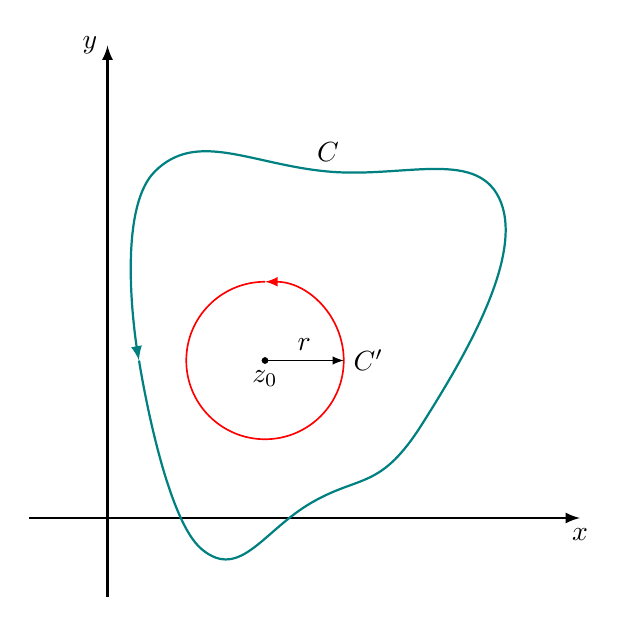
\begin{tikzpicture}[scale=2.0]
    \usetikzlibrary {arrows.meta}
    \usetikzlibrary {calc}
    
    
    \draw [thick, -latex] (-0.5, 0) -- (3, 0) node[below] {$x$};
    \draw [thick, -latex] (0, -0.5) -- (0, 3) node[left] {$y$};
    
    \filldraw [] (1, 1.0) circle (0.5pt) node [below] {$z_0$} ;
    \coordinate (a1) at (0.2, 1.0);
    \coordinate (a2) at (0.6, -0.2);
    \coordinate (a3) at (1.3, 0.1);
    \coordinate (a4) at (2, 0.6);
    \coordinate (a5) at (2.5, 2.0);
    \coordinate (a6) at (1.4,2.2);
    \coordinate (a7) at (0.3 , 2.2);
    \coordinate (O) at ($(a1)-(1,2)$);
    \draw [teal, thick, -latex]  plot[smooth, tension=.8] coordinates {(a1) (a2) (a3) (a4) (a5) (a6) (a7) (a1)};
    \node[above] at (a6) {$C$};
    \draw[red, thick, -latex, semithick] (1.0, 1.5) arc (90:450:0.5);
    \draw[-latex] (1.0, 1.0) -- (1.5, 1.0);
    \node[right] at (1.5, 1.0) {$C'$};
    \node[above] at (1.25, 1.0) {$r$};
    %\filldraw [] (a1) circle (1pt) node [below] {$a_1$} ;
    %\filldraw [] (a2) circle (1pt) node [below] {$a_2$} ;
    %\filldraw [] (a3) circle (1pt) node [below] {$a_3$} ;
    %\filldraw [] (a4) circle (1pt) node [below] {$a_4$} ;
    %\filldraw [] (a5) circle (1pt) node [below] {$a_5$} ;
    %\filldraw [] (a6) circle (1pt) node [below] {$a_6$} ;
    %\filldraw [] (a7) circle (1pt) node [below] {$a_7$} ;
    \end{tikzpicture}
\end{document}